\newpage
\section{Auswertung}
\label{sec:Auswertung}

Zur Auswertung des Versuchs wurde für numerische Berechnungen das Programm Numpy \cite{numpy} und
für die Erstellung von Abbildungen das Programm matplotlib \cite{matplotlib} verwendet.
Die Berechnungen der Unsicherheiten wurde unter Verwendung von Uncertainties \cite{uncertainties}
durchgeführt und einzelne im Folgenden näher beschriebene Funktionen des
Pakets SciPy \cite{scipy} wurden verwendet.

\subsection{Eichung des Elektromagneten}
\label{sec:AuswEichung}

Die Stärke des angelegten Magnetfelds wird mit der Stärke des an den Elektromagneten angelegten
Feldstroms $I$ variiert.
Für nachfolgende Messungen wurde die magnetische Flussdichte $B$ deshalb geeicht.
Die zu diesem Zweck aufgenommenen Daten sind in Tabelle \ref{tab:eichung} dargestellt.
\input{build/eichung.tex}
An die Messwerte wurde mit der Funktion \texttt{curve\_fit} der Bibliothek
\texttt{scipy.optimize} eine Regression der Form
\begin{equation*}
  B\!\left(I\right) = a_0 + a_1 I + a_2 I^2 + a_3 I^3 + a_4 I^4
\end{equation*}
durchgeführt.
Die Parameter $a_\text{i}$ wurden auf
\begin{align*}
  a_0 &= \SI{9(3)}{\milli\tesla} \\
  a_1 &= \SI{54(2)}{\milli\tesla\per\ampere} \\
  a_2 &= \SI{1.4(5)}{\milli\tesla\per\ampere\squared} \\
  a_3 &= \SI{-0.08(3)}{\milli\tesla\per\raiseto{-3}\ampere} \\
  a_4 &= \SI{0.0001(9)}{\milli\tesla\per\raiseto{-4}\ampere} \\
\end{align*}
bestimmt.
Der Verlauf der Regression ist zusammen mit den aufgenommenen Messwerten in
Abbildung \ref{fig:eichung} dargestellt.

\begin{figure}
	\centering
	\includegraphics[height=8cm]{build/eichung.pdf}
	\caption{Aufgenommene Werte der magnetischen Flussdichte in Abhängigkeit des
	anglegten Stroms mit durchgängig dargestellter Regression.}
	\label{fig:eichung}
\end{figure}


\subsection{Analyse der roten Spektrallinie}
\label{sec:AuswRot}

\begin{figure}
  \centering
  \begin{subfigure}{.32\textwidth}
    \centering
    
\includegraphics[width=\textwidth]{rohdaten/rot_sigma_0A.JPG}
    \caption{$I = \SI{0}{\ampere}.$}
  \end{subfigure}
  \begin{subfigure}{.32\textwidth}
    \centering
    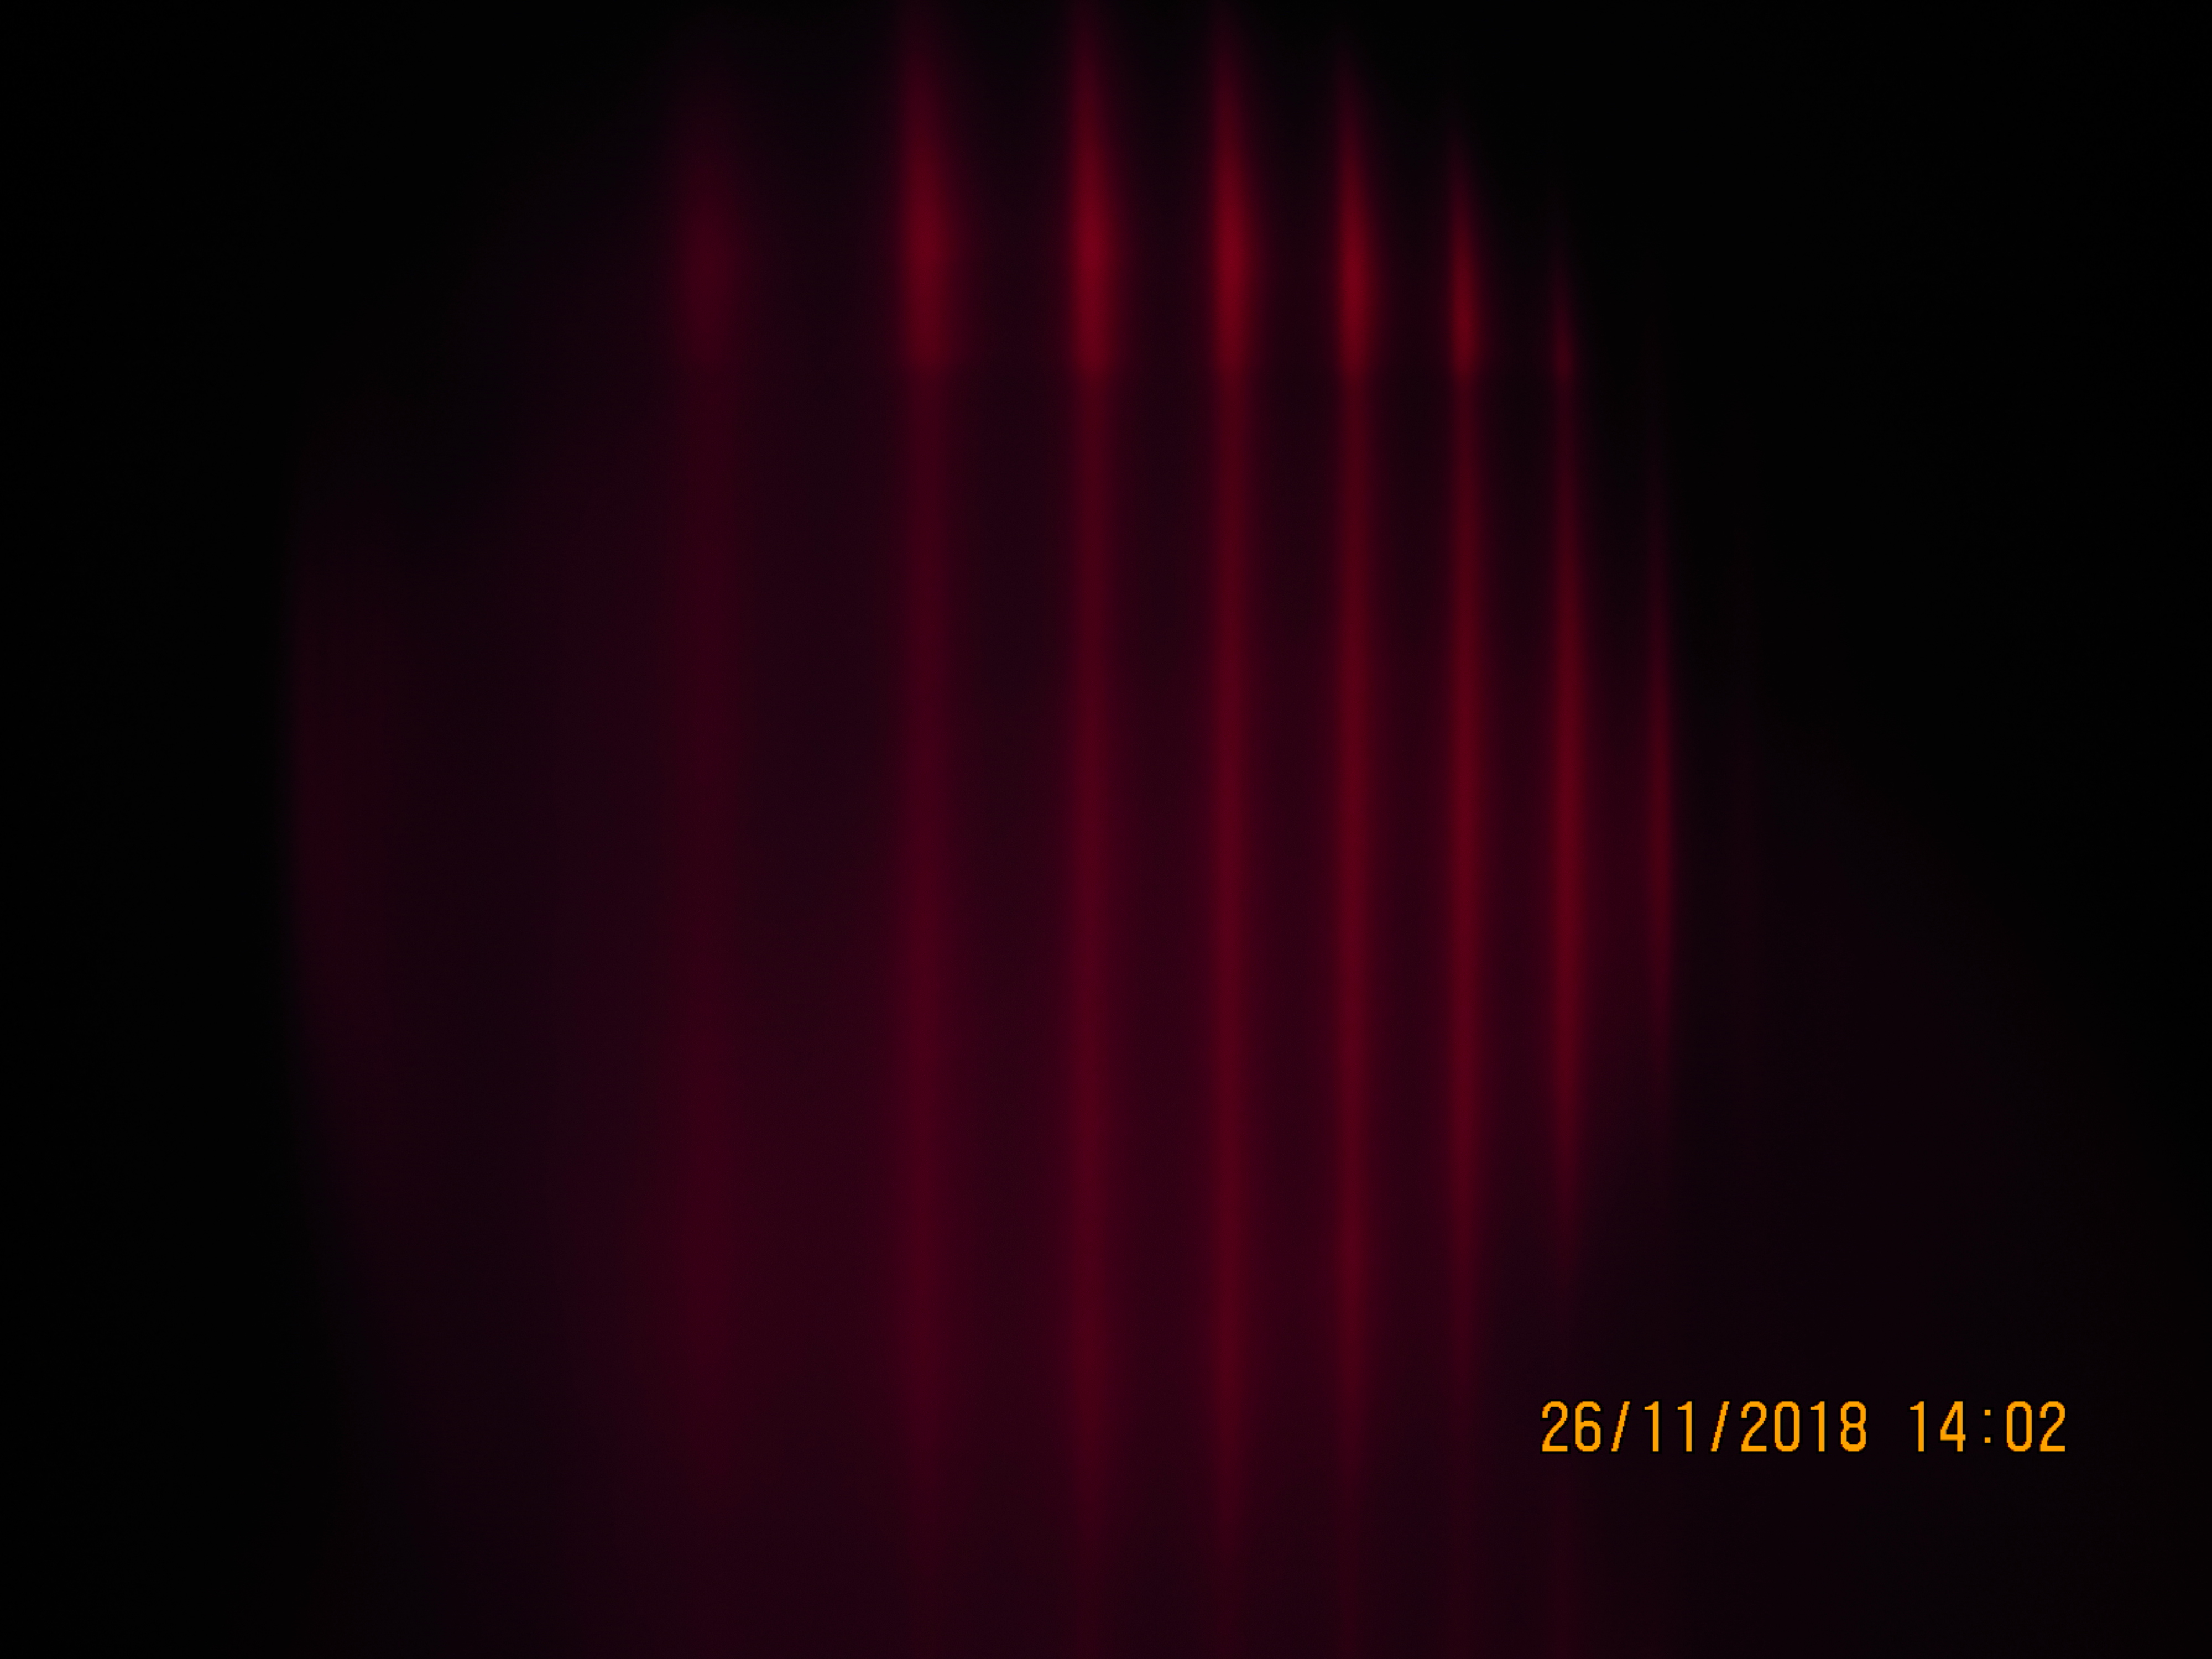
\includegraphics[width=\textwidth]{rohdaten/rot_pi_10,5A-2.JPG}
    \caption{$\pi$-Übergang bei $I = \SI{10.5}{\ampere}.$}
  \end{subfigure}
  \begin{subfigure}{.32\textwidth}
    \centering
    
\includegraphics[width=\textwidth]{rohdaten/rot_sigma_10,5A.JPG}
    \caption{$\sigma$-Übergang bei $I = \SI{10.5}{\ampere}.$}
  \end{subfigure}
  \caption{Die Linienaufspaltung der roten Spektrallinie.}
  \label{fig:AuswRot}
\end{figure}

Die aufgenommenen Bilder zur Linienaufspaltung der roten Spektrallinie sind in
Abbildung \ref{fig:AuswRot} dargestellt.
Dabei entspricht der Feldstrom von \SI{10.5}{\ampere} einer magnetischen
Flussdichte von \SI{0.64(7)}{\tesla}.
Wie in der Diskussion näher erläutert wird für die $\pi$-Linie keine Aufspaltung
erwartet. Dies konnte anhand der Bilder a) und b) verifiziert werden.
Für die $\sigma$-Linie ist in Abbildung \ref{fig:AuswRot} eine Aufspaltung
beobachtbar.
Zur näheren Untersuchung werden die Bilder b) und c) eingelesen und der rote
Anteil der RGB-Werte der Bilder näher betrachtet.
Der Verlauf eines horizontalen Schnitts entlang der Bilder b) und c) auf halber
Höhe sind in den Abbildungen \ref{fig:RotSigmaSchnitt}
und \ref{fig:RotPiSchnitt} dargestellt.

\begin{figure}
  \centering
  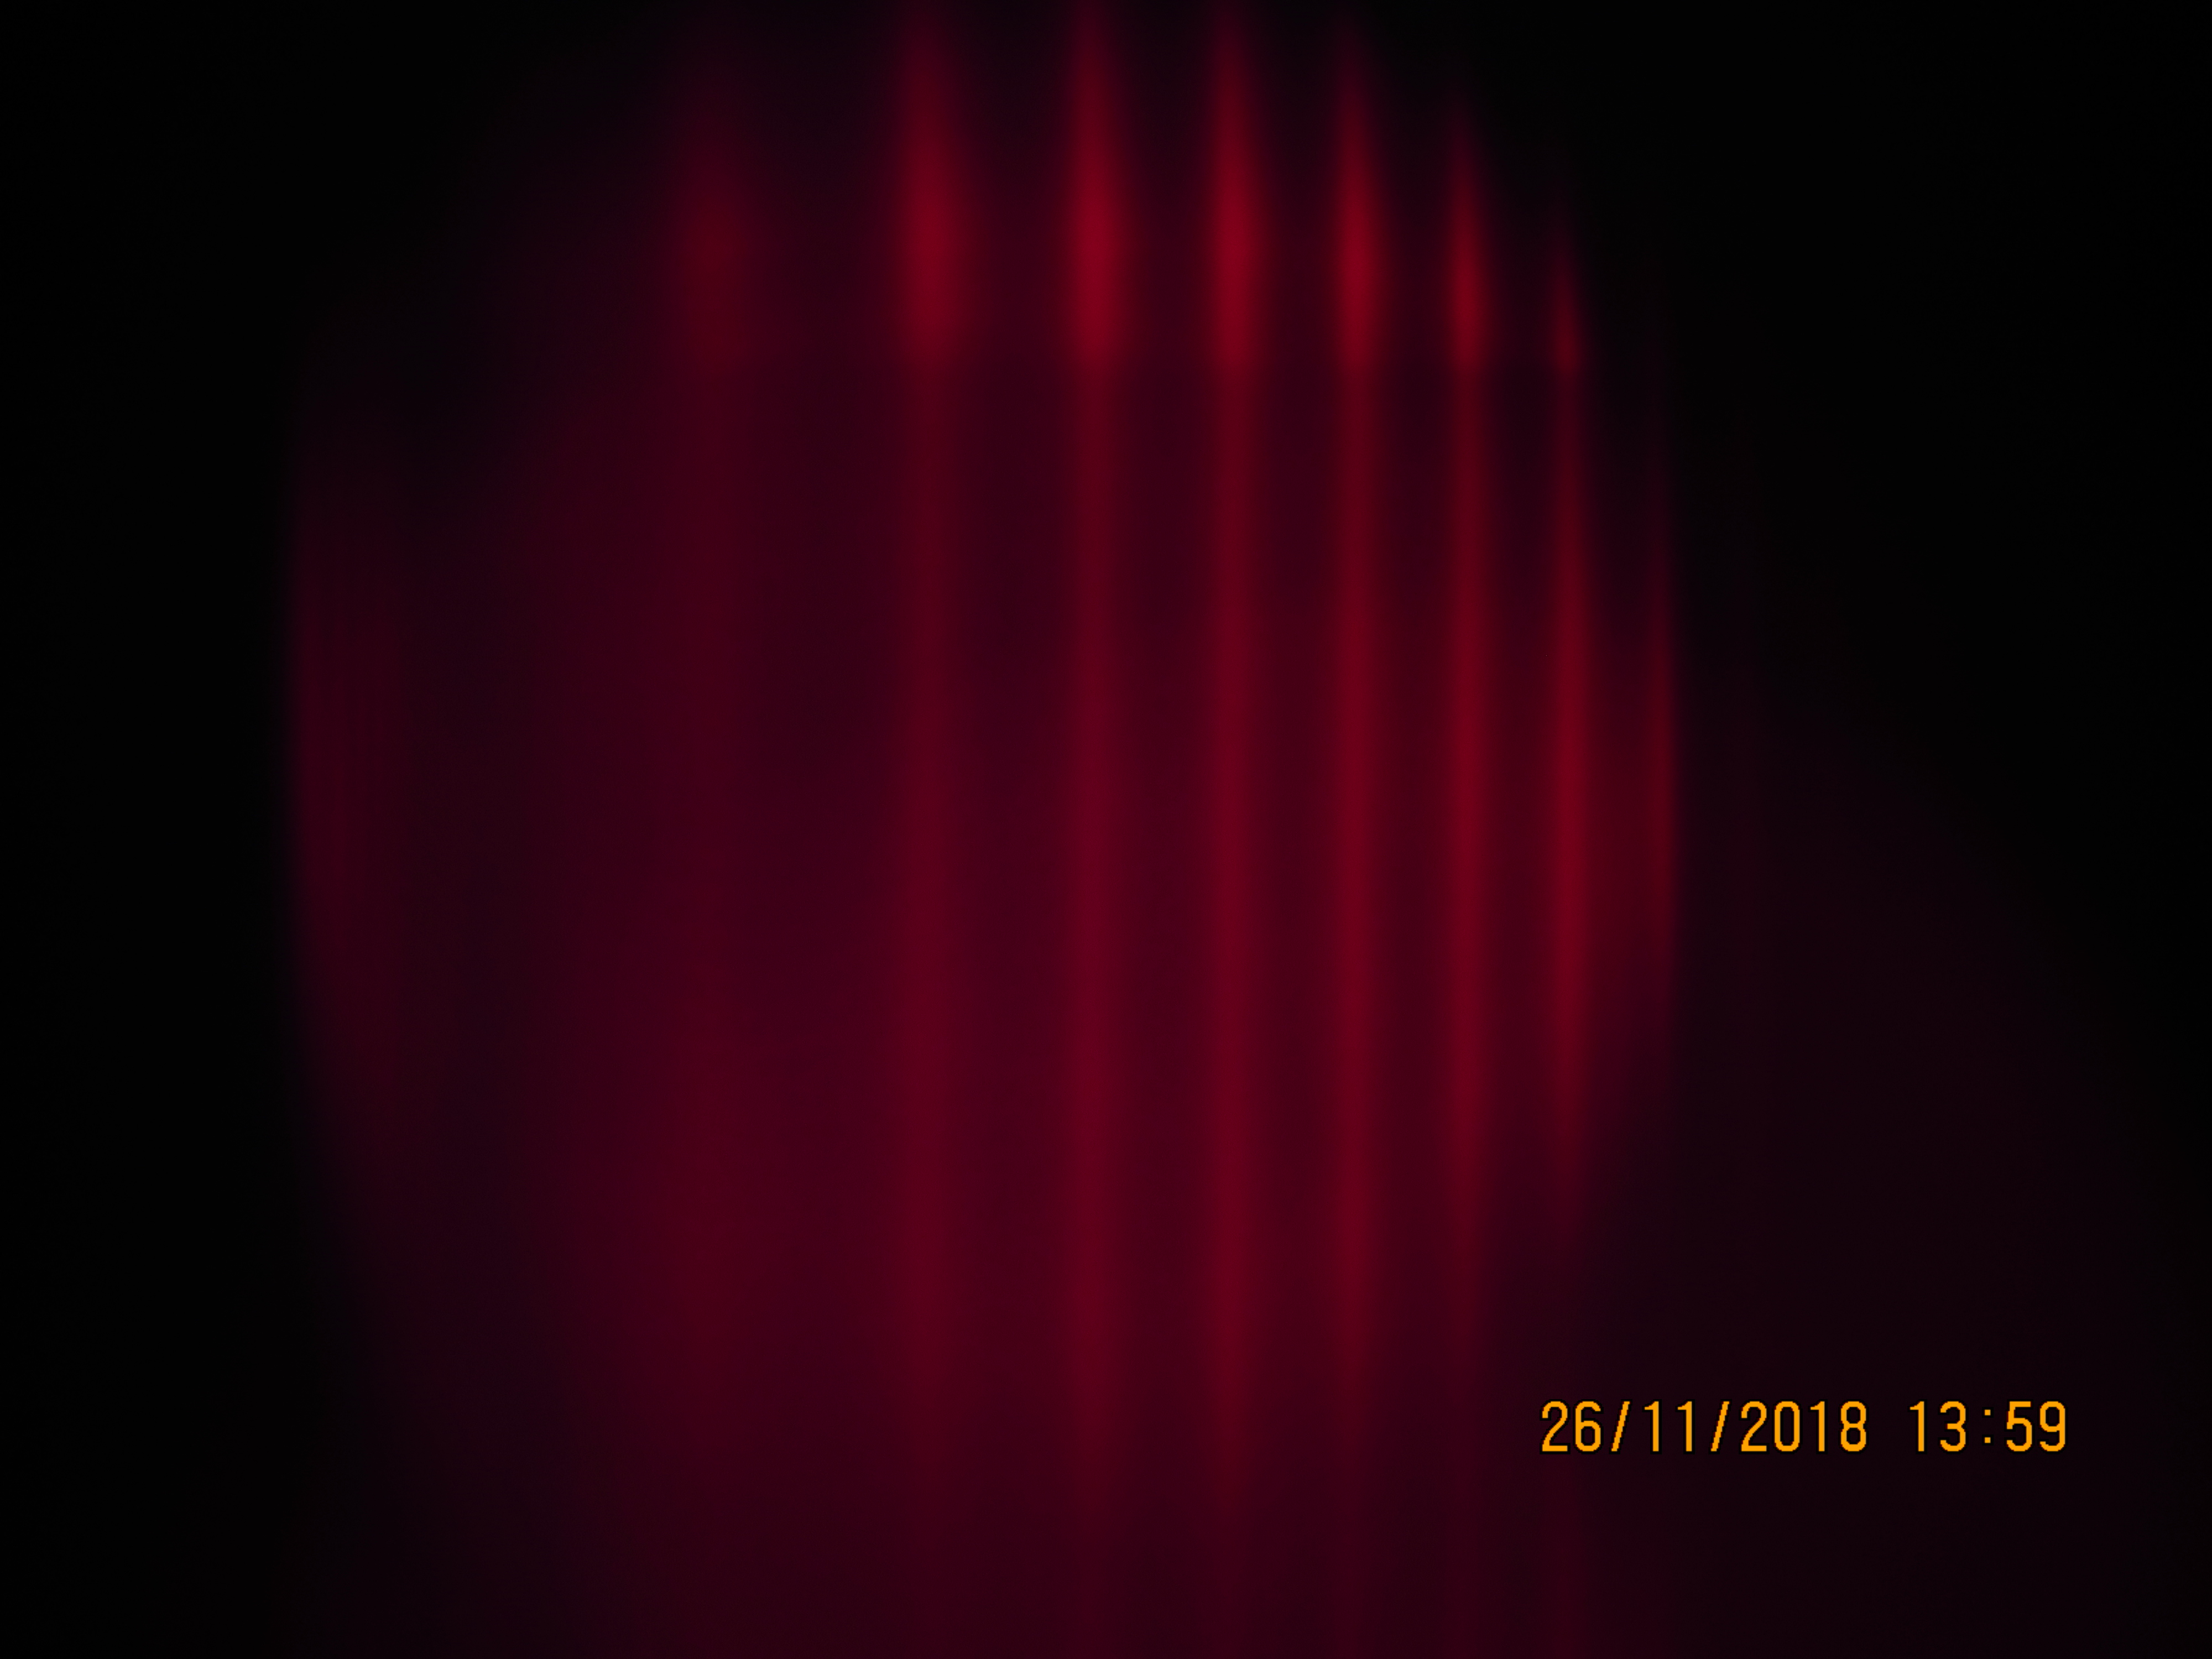
\includegraphics[height=8cm]{build/rot_pi_10,5A.pdf}
  \caption{Die Rotwerte eines horizontalen Schnitt des Bildes der
    $\pi$-Linie bei \SI{10.5}{\ampere}.}
  \label{fig:RotSigmaSchnitt}
\end{figure}
\begin{figure}
  \centering
  
\includegraphics[height=8cm]{build/rot_sigma_10,5A.pdf}
  \caption{Die Rotwerte eines horizontalen Schnitt des Bildes der
    $\sigma$-Linie bei \SI{10.5}{\ampere}.}
  \label{fig:RotPiSchnitt}
\end{figure}

Unter Verwendung der Funktion \texttt{find\_peaks} der Bibliothek \texttt{scipy.signal}
wurden für einen Bereich des Schnitts die Maxima des Verlaufs bestimmt.
Sie sind ebenfalls in den Abbildung \ref{fig:RotSigmaSchnitt} und \ref{fig:RotPiSchnitt}
als rote Kreuze dargestellt.
Diese Maxima stellen die roten Linien im Spektrum dar und und die Differenz dieser
lässt sich für Analyse der relativen Ausbreitung nutzen.
Es gilt für die Wellenlängenänderung $\delta\lambda$
\begin{equation}
  \delta\lambda = \frac{1}{2} \frac{\delta s}{\Delta s} \cdot \Delta \lambda_\text{D}
  \label{eqn:Wellenlaengenaenderung}
\end{equation}
mit dem Dispersionsgebiet $\Delta \lambda_\text{D}$ der Lummer-Gehrcke-Platte und
den Abständen der Maxima bei $I = \SI{0}{\ampere}$ ($\Delta s$) und
$I = \SI{10.5}{\ampere}$ ($\delta s$).

Aus der Wellenlängenänderung lässt sich der Lande-Faktor bestimmen.
Dazu wird die Änderung der Energie $E = \sfrac{h c}{\lambda}$ mit der
Lichtgeschwindigkeit $c$ und dem Planckschen Wirkungsquantum $h$
bei einer Änderung der Wellenlänge
\begin{equation}
  \delta E = - \frac{h c}{\lambda^2} \delta\lambda
\end{equation}
betrachtet und mit Relation \eqref{eqn:EnergieAufspaltung} verglichen.
Es ergibt sich der Ausdruck
\begin{equation}
  \zeta = \left|\Delta \left(m g\right)\right|
  = -\frac{1}{2} \frac{h c}{\lambda^2} \frac{1}{\mu_\text{B}} \delta\lambda
  \label{eqn:Auswerungsfunktion}
\end{equation}

Für die rote Linie der Cd-Lampe ergeben sich die in Tabelle \ref{tab:rot_sigma}
dargestellten Werte für die Linienaufspaltungen, die Wellenlängenänderung und
$\zeta$.
Der Mittelwert der $\zeta$-Werte wurde auf
\begin{equation*}
  \mean{\zeta} = \num{0.96(10)}
\end{equation*}
bestimmt.
\input{build/rot_sigma.tex}

\subsection{Analyse der blauen Spektrallinie}
\label{sec:AuswBlau}

\begin{figure}
  \centering
  \begin{subfigure}{.49\textwidth}
    \centering
    
\includegraphics[width=\textwidth]{rohdaten/blau_pi_0A.JPG}
    \caption{$\pi$-Übergang bei $I = \SI{0}{\ampere}.$}
  \end{subfigure}
  \begin{subfigure}{.49\textwidth}
    \centering
    
\includegraphics[width=\textwidth]{rohdaten/blau_pi_18A.JPG}
    \caption{$\pi$-Übergang bei $I = \SI{18}{\ampere}.$}
  \end{subfigure}
  \\
  \begin{subfigure}{.49\textwidth}
    \centering
    \includegraphics[width=\textwidth]{rohdaten/blau_sigma_0A.JPG}
    \caption{$\sigma$-Übergang bei $I = \SI{0}{\ampere}.$}
  \end{subfigure}
  \begin{subfigure}{.49\textwidth}
    \centering
    
\includegraphics[width=\textwidth]{rohdaten/blau_sigma_6A.JPG}
    \caption{$\sigma$-Übergang bei $I = \SI{6}{\ampere}.$}
  \end{subfigure}
  \caption{Die Linienaufspaltung der roten Spektrallinie.}
  \label{fig:AuswBlau}
\end{figure}

Die aufgenommenen Bilder zur Aufspaltung der blauen Linie der Cd-Lampe
sind in Abbildung \ref{fig:AuswBlau} dargestellt.
Dabei entspricht ein Feldstrom von \SI{18}{\ampere} einer magnetischen
Flussdichte von \SI{0.99(27)}{\tesla} und ein Strom von
\SI{6}{\ampere} entspricht \SI{0.64(7)}{\tesla}.
Da hier sowohl beim $\pi$- als auch beim $\sigma$-Übergang Änderungen
der Wellenlänge erwartet werden, sind alle vier Bilder eingelesen worden
und in den Abbildungen \ref{fig:BlauPiSchnitt1} bis \ref{fig:BlauSigmaSchnitt2}
dargestellt.

\begin{figure}
  \centering
  
\includegraphics[height=8cm]{build/blau_pi_0A.pdf}
  \caption{Die Blauwerte eines horizontalen Schnitt des Bildes der
    $\pi$-Linie bei \SI{0}{\ampere}.}
  \label{fig:BlauPiSchnitt1}
\end{figure}
\begin{figure}
  \centering
  
\includegraphics[height=8cm]{build/blau_pi_18A.pdf}
  \caption{Die Blauwerte eines horizontalen Schnitt des Bildes der
    $\pi$-Linie bei \SI{18}{\ampere}.}
  \label{fig:BlauPiSchnitt2}
\end{figure}
\begin{figure}
  \centering
  \includegraphics[height=8cm]{build/blau_sigma_0A.pdf}
  \caption{Die Blauwerte eines horizontalen Schnitt des Bildes der
    $\sigma$-Linie bei \SI{0}{\ampere}.}
  \label{fig:BlauSigmaSchnitt1}
\end{figure}
\begin{figure}
  \centering
  
\includegraphics[height=8cm]{build/blau_sigma_6A.pdf}
  \caption{Die Blauwerte eines horizontalen Schnitt des Bildes der
    $\sigma$-Linie bei \SI{6}{\ampere}.}
  \label{fig:BlauSigmaSchnitt2}
\end{figure}

Analog zur Auswertung der roten Spektrallinie wurde auch hier an die
Blauwerte der horizontalen Bildschnitte mit Hilfe der Funktion
\texttt{find\_peaks} die Position der Maxima bestimmt.
Daraus ließen sich nach der Formel \eqref{eqn:Wellenlaengenaenderung}
die Wellenlängenänderungen und aus Formel \eqref{eqn:Auswerungsfunktion}
die Werte für $\zeta$ bestimmen.
Sie sind in den Tabellen \ref{tab:blau_sigma} und \ref{tab:blau_pi} dargestellt.
Als Mittelwerte ergeben sich
\begin{align*}
  \mean{\zeta_{\pi}} &= \num{0.48(13)} \quad \text{und}\\
  \mean{\zeta_{\sigma}} &= \num{1.95(12)}. \\
\end{align*}
\input{build/blau_sigma.tex}
\input{build/blau_pi.tex}
